\section{Evaluation Design}
\label{sec:evaluation}
\subsection{Electrical and Charging Models}
The experiment uses the public IEEE 123-node and 13-node feeder definitions
distributed with OpenDSS~\cite{epriopendss}. Six phase-connected EV groups are
placed at buses 48.1, 76.2, 83.3, 67.1, 95.2, and 105.3 in the primary feeder.
The 13-node check uses 632.1, 671.2, 675.3, 680.1, 645.2, and 611.3.
These are unity-power-factor, medium-voltage equivalent loads; low-voltage
cables, charger harmonics, battery aging, and protection dynamics are not modeled.
Published background demand is first scaled to 80\%, then multiplied by a
scenario factor centered at 0.9 or 1.0 with a known $\pm0.01$ uncertainty
interval. Regulators initialize at a 120-V target and their taps remain fixed
during replay. Actual AC power flow is solved after each change in charging power
or background demand.

Each 30-min episode contains 156 synthetic sessions with staggered arrivals and
departures, heterogeneous requested energy, and constant 22-kW acceptance limits.
Group caps are at most 300~kW. The 13-node check scales these powers and requests
by $2/3$. Control and telemetry periods are 30~s; normal one-way delay is
2--2.9~s, and nominal actuation takes 1~s. Local EDF service integrates energy
exactly between arrival, completion, departure, actuation, and expiry events.
The persistent fallback is 65\% of each group's initial feasible cap.

The affine model uses operating points of 100~kW/group on IEEE 123 and
50~kW/group on IEEE 13. Development tightening is respectively 0.005 and
0.002~p.u. for voltage, with a 0.98 loading limit on both feeders. Independent
margin checks used 10\,000 random power/background draws per feeder and loading
center. The affine test admitted 9\,110/6\,860 draws on IEEE 123 and
9\,629/5\,999 on IEEE 13 at centers 0.9/1.0, with no admitted AC violation.
This finite check informs the selected margins; it supplies no global AC guarantee.
Replay limits remain 0.95--1.05~p.u. voltage and unity transformer terminal-phase
current loading.

\subsection{Channel Conditions and Comparators}
The clean condition has only normal delay. T1 drops messages on three affected
group links during a staggered 270--716~s window. T2 delays affected reductions
until reconnection and adds 45~s to application-certificate delivery during the
window. T3 delays affected increases until 180~s after reconnection, retaining
possible late execution; certificates again incur the extra delay. T4 delays
commands and queries around 900-s profile expiry, when a temporary low cap can
revert to a higher fallback. The exact per-group offsets, queue rules, and
absolute validity times are fixed in the companion configuration files.
These are distinct stress conditions, not matched random-versus-selective
attack distributions. The attacker controls the specified channel timing or
availability, not authenticated command contents, the adapter, or its truthful
post-application evidence.
Selective cases grant observation of command direction at the messaging layer.
This is an adversary-capability assumption; encrypted-transport compromise and
charger exploitation are outside the model.

Seven policies share these physical and information interfaces. B0 reallocates
as if requested caps immediately apply. B1 guards allocation using the latest
measured and requested power with headroom, without retaining the full execution
history. Its headroom was selected from 5\%, 10\%, and 20\% on 50 development
cases, choosing the smallest setting with zero observed electrical violations:
20\%. B2 keeps the initial static feasible quotas. The serialized ledger variant
B3 uses the execution ledger
with per-group stop-and-wait and repeated state queries; an unresolved command
blocks new commands until evidence or absolute expiry resolves it. Neither B3
nor P retransmits commands in the primary experiment. B4 uses a minimum-peak,
deadline-energy linear program to form
capacity-sharing requests, followed by the same serialization and feeder checks.
It is inspired by dynamic capacity sharing~\cite{gumrukcu2024dcs}, not a
reproduction of that work's peer protocol or restoration objective. P permits
the nonexpanding supersession of Section~\ref{sec:filter}. R gives P immediate
truthful application certificates but retains forward-channel delay and common
energy telemetry; it is not an omniscient service bound.

\subsection{Pairing, Metrics, and Ablations}
The primary study has 30 independently generated cohorts, five channel
conditions, two loading centers, and seven policies: 2\,100 episodes.
The main impaired analysis contains 240 episodes per policy
(Table~\ref{tab:main}); the 60 clean episodes are separate.
Another 840 episodes use ten new cohort seeds with
12 settings: certificate-delay extensions of 15/90/180~s, one/two/four affected
groups, actuation lags of 0/5/15~s, and the three IEEE 13 T1--T3 checks.
Finally, 80 ablation episodes remove pending-command accounting, remove fallback
accounting, credit acceptance as application, or substitute a scalar aggregate
budget for locational admission rows. Their matching full-P results come from
five main cohorts at the higher loading center.

Service is energy delivered before departure; shortfall is requested energy
minus that delivery. Safety metrics are the number of episodes with an actual
AC limit violation, violation duration, and integrated excess voltage/loading.
The primary paired P$-$B3 difference first averages the eight impaired conditions
within each cohort. A 10\,000-draw percentile bootstrap resamples the 30 cohort
blocks, preserving all paired conditions, to obtain a 95\% interval. Sensitivity
and ablation estimates retain their ten- and five-cohort units, respectively.
No timestep is an independent statistical sample. All controller settings and
evaluation seeds were fixed after development and before evaluation outputs.

The primary ledger variants do not retransmit lost commands. A supplementary
retry experiment, specified after the primary analysis and frozen before its
outcomes were examined, uses 30 new cohorts,
four impairments, two loads, and P/B3 with and without retries: 960 episodes.
Both retry variants resend their latest unresolved generation every 60~s when
no new command uses that group's remote procedure call (RPC) slot.
Cap, generation, and absolute lease
remain unchanged; duplicate receipt cannot reapply an accepted generation.
Retries retain their original command direction for T2/T3 classification and
replace a query on that tick. This follow-up is separate from the primary
analysis and uses the same cohort-block inference.

\section{Results and Discussion}
\label{sec:results}
\subsection{Electrical Outcomes and Service}
All 3\,980 episodes completed with converged AC solutions.
In the main impaired cases, P delivers
480.1~kWh/episode, 99.84~kWh more than B2 (95\% paired interval
$[95.94,103.87]$~kWh), a 26.3\% increase. B2, B3, B4, P, and R have no
observed electrical violations. P's worst voltage is 0.95487~p.u. and its
largest terminal-phase current loading is 0.98299~p.u.; no cap-containment
failure occurs. These are observed outcomes within the modeled conditions.

\begin{table}[t]
\caption{Impaired Main Results: 240 Episodes per Policy. Energy and Shortfall
Are Means; Loading Is the Worst Terminal-Phase Current Ratio.}
\label{tab:main}
\centering
\begin{tabular}{lrrrr}
\hline
Policy & Energy & Shortfall & Unsafe & Peak load \\
 & (kWh) & (kWh) & (/240) & (p.u.) \\
\hline
B0 & 546.2 & 222.9 & 192 & 1.120 \\
B1 & 355.8 & 413.3 & 22 & 1.043 \\
B2 & 380.3 & 388.8 & 0 & 0.980 \\
B3 & 482.6 & 286.4 & 0 & 0.980 \\
B4 & 466.9 & 302.2 & 0 & 0.977 \\
P & 480.1 & 288.9 & 0 & 0.983 \\
R & 481.9 & 287.2 & 0 & 0.983 \\
\hline
\end{tabular}

\end{table}

B0's greater delivery accompanies violations in 192 episodes, a minimum
voltage of 0.93772~p.u., and a maximum loading of 1.11963~p.u.
Even the clean condition produces 34/60 violating B0 episodes: ordinary
latency already makes immediate capacity release unreliable. Additional
impairment is therefore not the sole cause of this failure. B1's 20\% margin,
selected with zero development violations, yields 22/240 impaired and 2/60
clean violating cases. Sixteen impaired violations occur in T4, illustrating
that development headroom does not certify expiry-aware capacity release.

\subsection{Supersession Has a Service Cost}
P does not dominate the query-only serialized variant. Its paired mean
P$-$B3 difference is $-2.48$~kWh (95\% interval $[-3.23,-1.69]$), or
$-0.51\%$ relative to B3. Fig.~\ref{fig:paired} shows a negative effect
in T1 and T2, an interval spanning zero in T3, and a small positive T4
effect of 0.135~kWh. In the clean condition, B3, P, and R have identical
489.74-kWh mean delivery. Thus the measured service penalty emerges when
the policies interact with unresolved execution.

\begin{figure}[t]
\centering
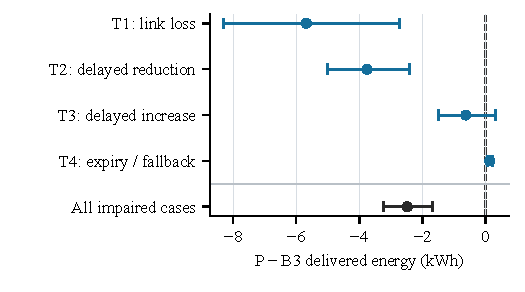
\includegraphics[width=\columnwidth]{paired_effects.pdf}
\caption{Paired supersession-minus-serialization energy differences. The 95\%
intervals resample 30 cohort blocks; each condition retains both loading levels.
Negative values favor B3.}
\label{fig:paired}
\end{figure}

P issues more commands than B3 (86.3 versus 68.1 per impaired episode) but
fewer queries (25.6 versus 49.1). Its integrated reserved-but-unused capacity
is smaller, 16.89 versus 22.19~kWh-equivalent, without greater delivered
energy. Reservation slack alone is therefore not a service objective.
Fig.~\ref{fig:trace} presents the prespecified median-effect T1 example,
selected across all 30 higher-loading cohorts. P delivers 9.43~kWh less
than B3 in this case.
R improves P's mean delivery to 481.9~kWh, but remains below B3; immediate
application evidence is not a service upper bound for a greedy scheduler.

\begin{figure}[t]
\centering
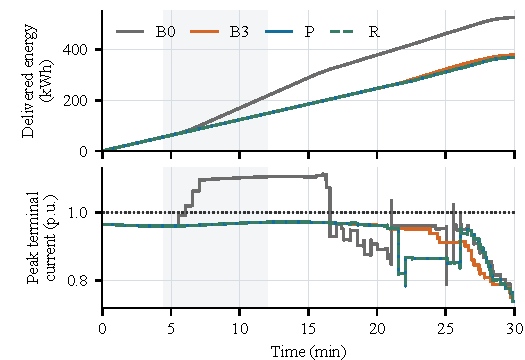
\includegraphics[width=\columnwidth]{representative_trace.pdf}
\caption{Median-effect T1 example (cohort 1011, loading center 1.0).
Curves show actual delivered energy and transformer terminal-phase loading.
The shaded interval spans the staggered link outages. All trace replays
reproduce their saved main-case metrics.}
\label{fig:trace}
\end{figure}

\subsection{Supplementary Retry Comparison}
Table~\ref{tab:retry} reports the separately frozen 960-episode follow-up. All four
implementations have zero electrical violations or cap-containment failures.
With retries enabled for both, P$_{\mathrm r}-$B3$_{\mathrm r}$ is
$-0.825$~kWh (95\% interval $[-1.137,-0.497]$), or $-0.17\%$.
On these same new cohorts, the query-only difference is $-2.406$~kWh.
Thus equal retry capability narrows the aggregate gap without establishing a
supersession service advantage. Retry-enabled P gains 0.400~kWh relative to
retry-enabled B3 in T1, while losing 3.370~kWh in T2.

\begin{table}[t]
\caption{Supplementary Retry Experiment: 240 Episodes per Policy.
Subscript r Denotes 60-s Same-Generation Retries.
Commands Include Retransmissions.}
\label{tab:retry}
\centering
% Post-review robustness experiment on new cohorts; initial primary analysis unchanged.
\begin{tabular}{lrrrr}
\hline
Policy & Energy & Unsafe & Commands & Queries \\
 & (kWh) & (/240) & (mean) & (mean) \\
\hline
B3 & 484.7 & 0 & 67.9 & 49.0 \\
P & 482.3 & 0 & 85.1 & 26.1 \\
B3$_{\mathrm{r}}$ & 483.0 & 0 & 93.6 & 12.9 \\
P$_{\mathrm{r}}$ & 482.2 & 0 & 93.6 & 10.0 \\
\hline
\end{tabular}

\end{table}

Retries are not guaranteed to improve this service metric: B3$_{\mathrm r}-$B3
is $-1.680$~kWh, while P$_{\mathrm r}-$P is $-0.099$~kWh with an interval
spanning zero. Retry attempts consume RPC opportunities otherwise available
for state queries and alter subsequent greedy reallocations. The measured
comparison supports the reservation accounting under both communication
strategies, without recommending either as an optimal scheduling policy.

\subsection{Sensitivity, Ablations, and Scope}
P and B3 remain violation-free in all 120 sensitivity cases per policy,
giving 420/420 when combined with their main cases. Longer evidence delay
can change service: at a 180-s certificate-delay extension, P$-$B3 is
$-3.15$~kWh with interval $[-5.56,-0.22]$. The 13-node checks also preserve
electrical feasibility; they do not establish topology-independent guarantees.
Across the 20 cases per ablation, omitting fallback accounting produces four
violating episodes and replacing locational admission with an aggregate budget
produces nine. Omitting pending-command accounting or crediting acceptance
produces no AC violation in these sampled cases. These null outcomes do not
establish that either omission is safe; they limit the empirical necessity
claim for those mechanisms. Both safeguards remain assumptions of the formal
result and are covered by execution-level regression tests.

On the recorded shared execution host, the median of episode-level median
filter times is 0.773~ms for P and 0.619~ms for B3; observed maxima are
37.88 and 15.28~ms. These exclude AC replay and communication, and are not
real-time implementation guarantees. Source, frozen scenarios, raw episode data,
analysis scripts, and editable SVG figures are available at
\url{https://github.com/asayghe1/ev-charging-cyber-resilient-recovery}.
Synthetic demand, fixed acceptance limits, static feeder controls, and the
trusted adapter restrict external validity. The implemented serialization
variant provides greater aggregate service in the primary study; supersession
is an option under the same reservations with condition-dependent service
effects. This comparison does not establish an optimal production recovery policy.

